\documentclass{article}

% if you need to pass options to natbib, use, e.g.:
%     \PassOptionsToPackage{numbers, compress}{natbib}
% before loading neurips_2018

% ready for submission
%\usepackage{neurips_2018}

% to compile a preprint version, e.g., for submission to arXiv, add add the
% [preprint] option:
\usepackage[preprint]{neurips_2018}

% to compile a camera-ready version, add the [final] option, e.g.:
%\usepackage[final]{neurips_2018}

% to avoid loading the natbib package, add option nonatbib:
%     \usepackage[nonatbib]{neurips_2018}

\usepackage[utf8]{inputenc} % allow utf-8 input
\usepackage[T1]{fontenc}    % use 8-bit T1 fonts
\usepackage{hyperref}       % hyperlinks
\usepackage{url}            % simple URL typesetting
\usepackage{booktabs}       % professional-quality tables
\usepackage{amsfonts}       % blackboard math symbols
\usepackage{nicefrac}       % compact symbols for 1/2, etc.
\usepackage{microtype}      % microtypography
\usepackage{epsfig}
\usepackage{graphicx}
\usepackage{xcolor}

\usepackage{amsfonts,amsmath,amssymb,amsthm}
\usepackage{bm,nicefrac}

\title{ECNet: Early Attention and Local Convolution for Machine Comprehension}

% The \author macro works with any number of authors. There are two commands
% used to separate the names and addresses of multiple authors: \And and \AND.
%
% Using \And between authors leaves it to LaTeX to determine where to break the
% lines. Using \AND forces a line break at that point. So, if LaTeX puts 3 of 4
% authors names on the first line, and the last on the second line, try using
% \AND instead of \And before the third author name.

\author{%
  %David S.~Hippocampus\thanks{Use footnote for providing further information
    %about author (webpage, alternative address)---\emph{not} for acknowledging
    %funding agencies.} \\
  %Department of Computer Science\\
  %Cranberry-Lemon University\\
  %Pittsburgh, PA 15213 \\
  %\texttt{hippo@cs.cranberry-lemon.edu} \\
	Abhishek Goswami\\
  Microsoft\\
  Redmond, WA 98052 \\
  \texttt{agoswami@microsoft.com} \\
  % examples of more authors
  % \And
  % Coauthor \\
  % Affiliation \\
  % Address \\
  % \texttt{email} \\
  % \AND
  % Coauthor \\
  % Affiliation \\
  % Address \\
  % \texttt{email} \\
  % \And
  % Coauthor \\
  % Affiliation \\
  % Address \\
  % \texttt{email} \\
  % \And
  % Coauthor \\
  % Affiliation \\
  % Address \\
  % \texttt{email} \\
}

\begin{document}
% \nipsfinalcopy is no longer used

\maketitle

\begin{abstract}

Current state-of-the-art machine comprehension models have some common tenets. One, the use of an embedding encoder layer to exploit contextual cues from surrounding words. Two, the use of neural attention mechanisms to exploit matching cues between the context and the query. In this paper we propose ECNet, a hierarchical model for machine comprehension, which amplifies existing models by adding early attention and local convolution. It uses self-attention over the input embeddings as a form of early attention. For the embedding encoder layer, ECNet models both sequential and local interactions between words, using recurrent and convolution layers respectively and combining them.  On the SQuAD 2.0 dataset, ECNet outperforms the BiDAF model proposed recently in literature.

\end{abstract}

\section{Introduction}
\label{sec:introduction}

Machine comprehension (MC) and question answering (QA) tasks have gained significant interest in the past few years, with several end-to-end models showing promising results for multiple datasets. A key factor in recent advancements has been the use of neural attention mechanisms. They fundamental idea behind attention is extract useful signal by exploiting the notion of \textit{matching}. 

Several attention approaches have been proposed in literature. Chen et al \cite{chen2016thorough} propose a \textit{uni-directional} attention mechanism whereby the query is used to attend to the context paragraph. In BiDAF, Seo at al \cite{seo2016bidirectional} introduce \textsl{bi-directional} attention flow to obtain a query-aware context representation. This provides complimentary information from both the context and query. Wang et al \cite{wang2017gated} note that question-aware passage representations have limited knowledge of the context itself. There exists some sort of lexical and syntactic difference between the question and the passage. This motivates them to directly match the question-aware passage representation against itself as a form of \textit{self-matching} attention. 

Another key tenet of the proposed techniques is to use a model to process sequential inputs. This is typically done in the form of an embedding encoder layer. While recurrent neural networks have been the model of choice for this, recent work by Yu et al \cite{yu2018qanet} propose using a convolution and self-attention mechanism instead. 

In this project we explore two novel extensions. First, we observe that most existing models dive straight into the encoding layer, given the sequential inputs. Attention is an afterthought. One problem of such a representation is that it strains the embedding encoder layer, since the rest of the modeling layers are all stacked on top of it. We propose adding a `Base Attention Layer' as a form of self-attention over the raw word and character input embeddings and explore whether that improves model performance. Second, we explore whether we can have a contextual embed layer that uses a combination of recurrent layers and convolution layers. The motivation behind this is to bring the best of both worlds in the contextual embedding space.

 







\section{Model}
\label{sec:model}

In this section, we first formulate the machine comprehension problem and then describe the model. We adopt the following terminology. Let $N$ be the length of the context and $M$ be the length of the question. $D$ is the embedding size and $H$ is the hidden size of the model.


\subsection{Problem Statement}
\label{subsec:problemstatement}

The machine comprehension task considered in this paper is as follows. Given a context paragraph with N words C = \{$c_1$, $c_2$, ..., $c_N$\} and a query sentence with M words Q = \{$q_1$, $q_2$, ... $q_M$\} output a span S = \{$c_i$, $c_{i+1}$,...${c_{i+j}}$\} from the original paragraph C. 

\begin{table}[htbp]
    \caption{An example of a machine comprehension task.}
    \label{table:economicSchools} 
    \centering
    \begin{tabular}{|l|p{0.8\linewidth}|}
    \hline
    Question   &  Economy, Energy and Tourism is one of the what? \tabularnewline \hline
    Context  & Subject Committees are established at the beginning of each parliamentary session, and again the members on each committee reflect the balance of parties across Parliament. Typically each committee corresponds with one (or more) of the departments (or ministries) of the Scottish Government. The \textcolor{blue}{current Subject Committees} in the fourth Session are: Economy, Energy and Tourism; Education and Culture; Health and Sport; Justice; Local Government and Regeneration; Rural Affairs, Climate Change and Environment; Welfare Reform; and Infrastructure and Capital Investment \tabularnewline \hline
    Answer   & current Subject Committees \tabularnewline \hline
    \end{tabular}
 
\end{table}

\subsection{Model Overview}
\label{subsec:models}

Several state-of-the-art machine comprehension models have a similar structure. They have an embedding layer, an embedding encoder layer, a context-query attention layer, a model encoder layer and an output layer. We introduce two novel extensions to this structure.  One, we add a Embedding Attention Layer as a form of self-attention over the embedding layer and show that it indeed improves model performance. Second, for the embedding encoder layer we use a combination of recurrent and convolution operations. 

Thus, our machine comprehension model is a hierarchical multi-stage process consisting of six layers. 

\begin{enumerate}
\item \textbf{Embedding Layer}. This layer is a mix of character embedding and word embeddings. 
\item \textbf{Embedding Attention Layer}
\item \textbf{Embedding Encoder Layer}
\item \textbf{Attention Flow Layer}
\item \textbf{Model Encoder Layer} blah blah
\item \textbf{Output Layer} blah blah
\end{enumerate}

The details of each of the layers are as follows.

\paragraph{1. Embedding Layer.} In this layer we mix character embeddings with word embeddings. 

For character embeddings, we use a method similar to that proposed by Kim et al \cite{kim2016character}. We first convert a word to its character indices. We then pad (or truncate) each word so it has length $m_{word}$.  For each of these characters we lookup a dense character embedding (which has shape ${e_{char}}$). To combine the character embeddings, we use 1-dimensional convolutions over $m_{word}$ using ${e_{char}}$ as the input channel size. The output of the CNN are max-pooled over the entire width to obtain a fixed-size vector of shape ${e_{word}}$ for each word. 

For word embeddings, we use pre-trained word vectors from GloVe \cite{} to obtain the fixed embedding for each word. The size of the word embeddings is ${e_{word}}$ which is the same as the shape of the character-level embeddings for each word.  


\paragraph{2. Embedding Attention Layer.} Several state-of-the-art machine comprehension models have a similar structure. They have an embedding layer, an embedding encoder layer, a context-query attention layer, a model encoder layer and an output layer. We introduce two novel extensions to this structure.  One, we add a `Base Attention Layer` as a form of self-attention over the embedding layer and show that it indeed improves model performance. Second, for the embedding encoder layer we use a combination of recurrent and convolution operations. 

\paragraph{3. Embedding Encoder Layer.} Several state-of-the-art machine comprehension models have a similar structure. They have an embedding layer, an embedding encoder layer, a context-query attention layer, a model encoder layer and an output layer. We introduce two novel extensions to this structure.  One, we add a `Base Attention Layer` as a form of self-attention over the embedding layer and show that it indeed improves model performance. Second, for the embedding encoder layer we use a combination of recurrent and convolution operations. 

\paragraph{4. Attention Flow Layer.} Several state-of-the-art machine comprehension models have a similar structure. They have an embedding layer, an embedding encoder layer, a context-query attention layer, a model encoder layer and an output layer. We introduce two novel extensions to this structure.  One, we add a `Base Attention Layer` as a form of self-attention over the embedding layer and show that it indeed improves model performance. Second, for the embedding encoder layer we use a combination of recurrent and convolution operations. 

\paragraph{5. Model Encoder Layer.} Several state-of-the-art machine comprehension models have a similar structure. They have an embedding layer, an embedding encoder layer, a context-query attention layer, a model encoder layer and an output layer. We introduce two novel extensions to this structure.  One, we add a `Base Attention Layer` as a form of self-attention over the embedding layer and show that it indeed improves model performance. Second, for the embedding encoder layer we use a combination of recurrent and convolution operations. 

\paragraph{6. Output Layer.} Several state-of-the-art machine comprehension models have a similar structure. They have an embedding layer, an embedding encoder layer, a context-query attention layer, a model encoder layer and an output layer. We introduce two novel extensions to this structure.  One, we add a `Base Attention Layer` as a form of self-attention over the embedding layer and show that it indeed improves model performance. Second, for the embedding encoder layer we use a combination of recurrent and convolution operations. 

\begin{figure*}[h!]
\centering
	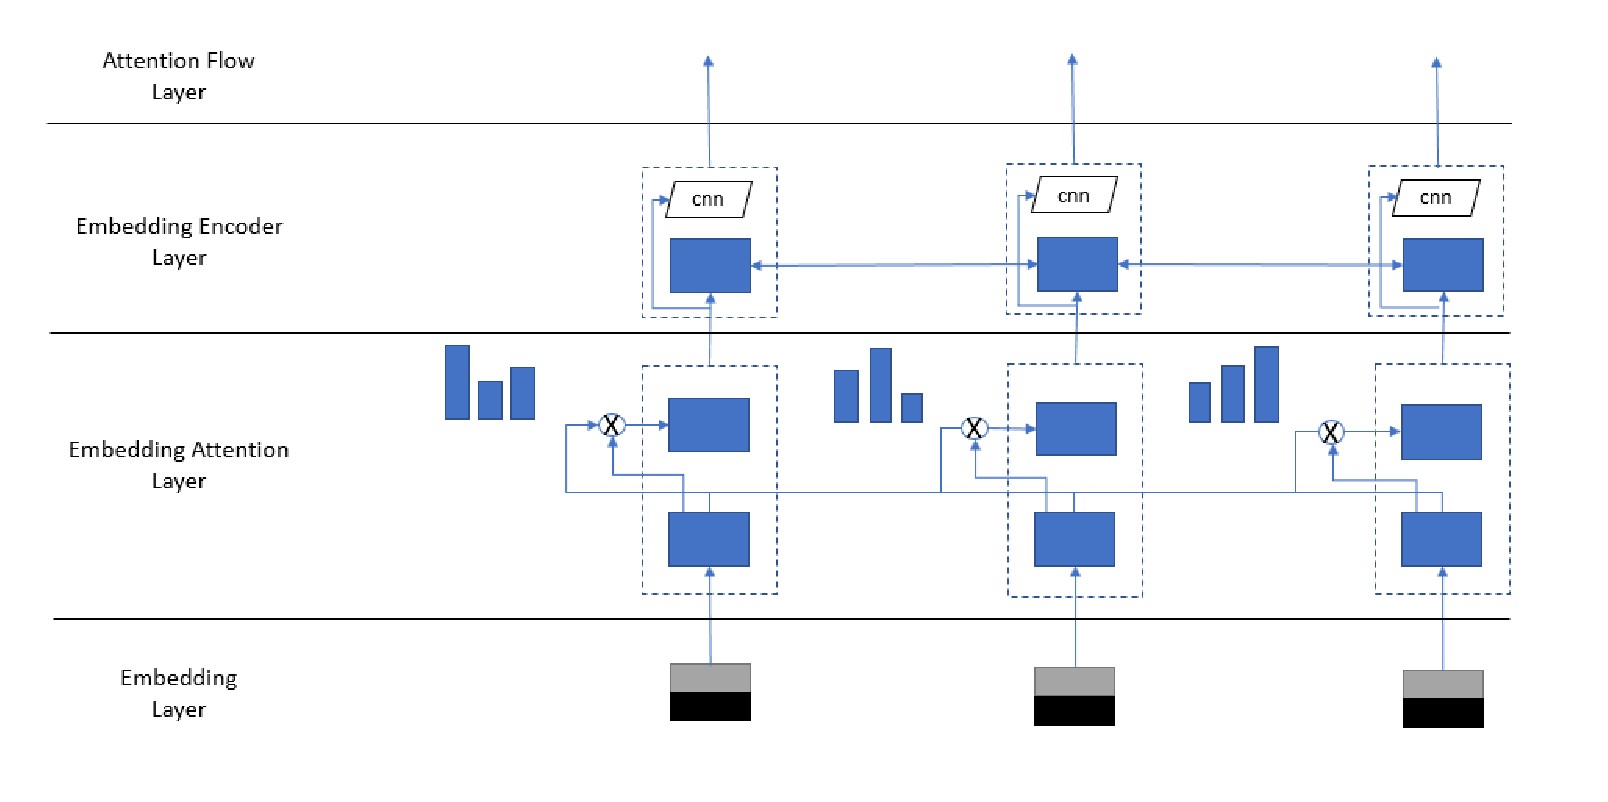
\includegraphics[width=12cm]{Figs4Paper/ModifiedLayers.eps}
  \caption{Convolutional network architecture}
  \label{fig:convnetarchitecture}
\end{figure*}

%\begin{figure*}[h!]
%\centering
	%\includegraphics[width=12cm]{Figs4Paper/EarlyAttentionLayer.eps}
  %\caption{Convolutional network architecture}
  %\label{fig:convnetarchitecture}
%\end{figure*}

\subsubsection{Base Attentional Model}
\label{subsubsec:baseattentionalmodel}

This model extends the baseline model by adding a `Base Attention Layer' as a form of self-attention over the raw word and character input embeddings. The motivation for adding this layer is two fold (a) the encoder layers could have missed some signal, hence  so just having post-attention layers may be insufficient (b) feed in more inputs from the input embed layers to the contextual embedding layers.


\subsubsection{RNN-Conv Contextual Embedding Model}
\label{subsubsec:rnnconvcontextualembeddingmodel}

This model extends the baseline model by having a contextual embedding layer that uses both RNN and Conv nets. The recurrent layers helps in processing sequential input, while convolution captures local structure of the text.  
\section{Experiment}
\label{sec:experiment}

In this section, we conduct experiments to study the performance of our models. We will benchmark our models on the Stanford Question Answering Dataset (SQuAD) 2.0 \cite{rajpurkar2018know}, considered to be one of the most competitive datasets in QA tasks. We also provide some implementation details for our models and present the main results.

\begin{figure*}[h!]
\centering
	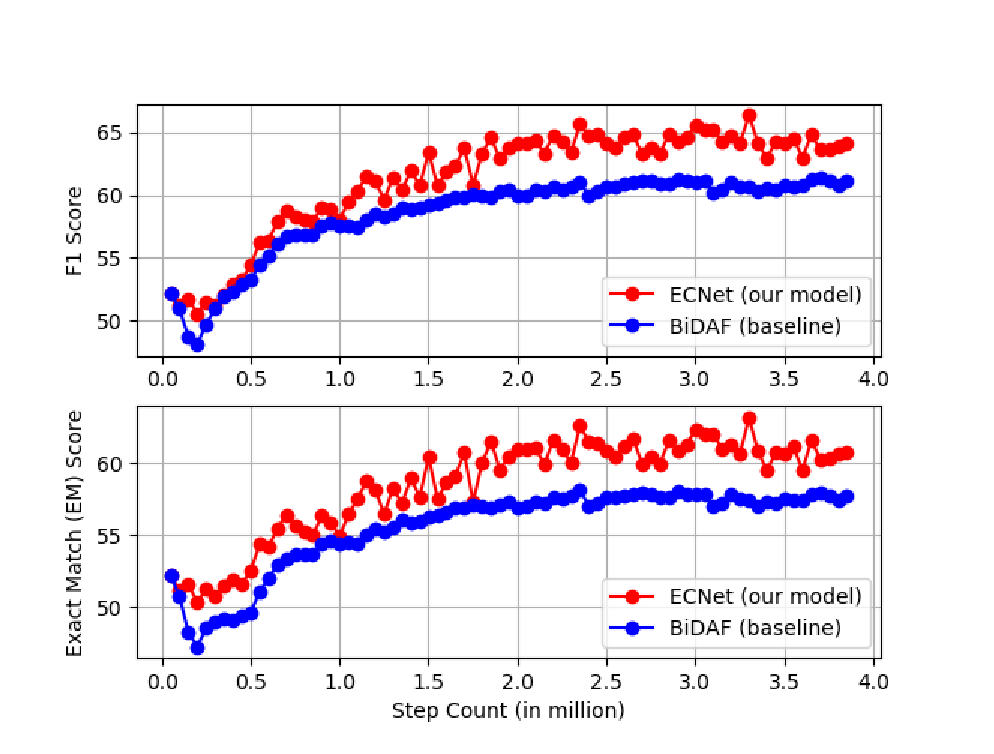
\includegraphics[width=12cm]{Figs4Paper/F1EM2.eps}
  \caption{Comparison of F1 and EM scores while training.}
  \label{fig:f1em}
\end{figure*}



\subsection{Dataset}
\label{subsec:dataset}

We consider the Stanford Question Answering Dataset (SQuAD) 2.0 \cite{rajpurkar2018know} for machine comprehension. Our model is given a paragraph, and a question about that paragraph, as input. The goal is to answer the question correctly. There are around 150k questions, and roughly half of the questions cannot be answered using the provided paragraph. 


\subsubsection{Data splits}
\label{subsubsec:dataset}

The official SQuAD dataset has three splits: train, dev and test. The train and dev sets are publicly available and the test set is entirely secret. For this project we use a custom dev and test set obtained by splitting the official dev set in half. 

To summarize we have the following data splits:

\begin{itemize}
\item \textbf{Train}. 129,941 examples. All taken from the official SQuAD 2.0 training set.
\item \textbf{Dev}. 6,078 examples. Roughly half of the official dev set, randomly selected.
\item \textbf{Test}. 5,915 examples. The remaining examples from the official dev set.
\end{itemize}

From now on we refer to these splits as the train set, dev set and test set respectively. We will use the train set to train the model. We report the performance metrics on the dev set.

\subsection{Training Details}
\label{subsec:trainingdetails}

The model architecture used for this task is shown in Figure \ref{fig:modelarchitecture}. 

For the Embedding Layer, $m_{word}$ is set to 16. ${e_{char}}$ and ${e_{word}}$ are set to 64 and 300 respectively. We use one 1D filter for the CNN char embedding with a kernel size of 5. The hidden state $d$ of the model is 100. For the convolutions in the Embedding Encoder Layer, we use a set of 4 stacked CNN layers, each with input/output channels as $2d$ with a kernel size of 1 . We uses dropout as a form of regularization across all the six layers in our model. Table \ref{table:dropoutresults} shows the effect of dropout on our model performance. We use the Adadelta optimizer \cite{zeiler2012adadelta} with a learning rate of 0.5 which is kept fixed. While training we use a batch size of 64. When scoring, $L_{max}$ is set to 15.

We implement our model in Python using PyTorch \cite{pytorch}. The experiments are carried out on a Azure Data Science Virtual Machine (DSVM) \cite{dsvm} which has a NVIDIA Tesla K80 GPU.

\subsection{Metric Details}
\label{subsec:metricdetails}

We measure performance via two metrics: Exact Match (EM) and the F1 score.

\begin{itemize}
\item \textbf{Exact Match} is a binary measure (i.e. true/false) of whether the system output matches the ground truth answer exactly.
\item \textbf{F1} is the harmonic mean of precision and recall.
\item When a question has no answer, both the F1 and EM score are 1 if the model predicts no-answer, and 0 otherwise.
\item For questions that do have answers, when evaluating on the dev or test sets, we take the maximum F1 and EM scores across the three human-provided answers for that question.
\end{itemize}

\subsection{Results}
\label{subsec:results}

\begin{table}[]
\caption{Comparing ECNet with BiDAF}
\label{table:results}
\centering
\begin{tabular}{lll}
																									& EM    & F1    \\ \hline
BiDAF with character embedding (baseline)				  & 59.47 & 62.46 \\
ECNet (our model)																	& 63.17 & 66.38 \\ \hline

\end{tabular}
\end{table}

Table \ref{table:results} shows the comparison between our model and the baseline. As per the original BiDAF model, we include a character-level embedding layer using character-level convnets. This gives us a very strong baseline to compare with. We see ECNet outperforms BiDAF on both the F1 and EM metrics. Figure \ref{fig:f1em} shows a comparison of the metrics while training the two models.


\subsection{Ablation Study}
\label{subsec:ablationstudy}


\begin{table}[]
\caption{Results from Ablation Study}
\label{table:ablation}
\centering
\begin{tabular}{lll}
                                                                       & EM    & F1    \\ \hline
No Embedding Attention Layer                                           & 60.93 & 64.34 \\
No CNN layers inside the Embedding Encoder Layer                       & 59.64 & 63.10 \\
No character embedding in the Embedding Layer                          & 59.47 & 62.46 \\
Un-freezing the character and word embeddings in the Embedding Layer 	 & 62.19 & 65.39 \\ \hline

\end{tabular}
\end{table}


Table \ref{table:ablation} shows the performance of the model and its ablations on the dev set. Having an embedding attention layer helps model performance. This validates our hypothesis that adding attention layers early in the model stack should help performance. For ablating the effect of the CNN layers, we experiment by removing the CNN layers from the embedding encoder layer. CNN layers prove to be critical, with a drop of 3 points on both metrics when absent. Char embeddings in the embedding layer also play a crucial role, whereby word-level embeddings represent the semantics of each word as a whole, while char-level embeddings better handle out-of-vocab (OOV) or rare words. Interestingly we also see that un-freezing the char-level and word-level embeddings gives us slightly lower performance. It seems the model gives slightly worse results if we allow the backpropagation to happen all the way through the embedding layer. This shows the pre-loaded embeddings are quite good, fine-tuning these embeddings do not generalize well to unseen data in the dev set. 

\begin{table}[]
\caption{Effect of dropoput}
\label{table:dropoutresults}
\centering
\begin{tabular}{lll}
																	& EM    & F1    \\ \hline
No Dropout		   									& 60.41 & 63.46 \\
Dropout = 0.1    									& 62.06 & 65.39 \\ 
Dropout = 0.2 (chosen)		  			& 63.17 & 66.38 \\ 
Dropout = 0.3    									& 59.84 & 63.81 \\ 
Dropout = 0.4    									& 61.10 & 64.09 \\ \hline

\end{tabular}
\end{table}

Table \ref{table:ablation} shows the effect of dropout rates. The model overfits with low dropout rates.  High drop-out rates help in preventing overfitting, but lead to lower EM/F1 scores. We settle on 0.2 as the dropout rate since it gives the best results.

% -----------------------------------------------
%\subsection{Implementation Details}
%\label{subsec:implementationdetails}

%\begin{table}[]
%
    %\caption{Preliminary Results}
    %\label{table:results} 
    %\centering
		%
%\begin{tabular}{|l|l|l|l|l|}
%\hline
                                                                %& \multicolumn{2}{l|}{\textbf{Dev Set}} & \multicolumn{2}{l|}{\textbf{Test Set}} \\ \hline
                                                                %& EM                & F1                & EM                 & F1                \\ \hline
%master                        				                          & 59.25             & 62.28             & 59.47              & 62.46             \\ \hline
%baselinemodel\_selfsimilaritybeforeattention								 		& 58.83             & 62.05             & 57.47              & 60.87             \\ \hline
%baselinemodel\_selfsimilarityafterattention								 			& 59.45             & 62.95             & 59.45              & 62.95             \\ \hline
%conflict\_without\_for\_loops																 		& 55.67             & 59.19             & 55.67              & 59.19             \\ \hline
%embedding\_with\_self\_similarity                               & 59.64             & 63.10             & 59.64              & 63.10             \\ \hline
%embedding\_with\_self\_difference                               & 52.19             & 52.19             & 52.19              & 52.19             \\ \hline
%conv\_rnn\_embed\_layer							                  	        & 60.93             & 64.34             & 60.93              & 64.34             \\ \hline
%embedding\_with\_self\_similarity\_conv\_rnn (0.0)              & 62.19             & 65.26             & 60.41              & 63.46             \\ \hline
%embedding\_with\_self\_similarity\_conv\_rnn (0.1)              & 62.19             & 65.26             & 62.06              & 65.39             \\ \hline
%embedding\_with\_self\_similarity\_conv\_rnn (0.2)              & 62.19             & 65.26             & 62.19              & 65.26             \\ \hline
%embedding\_with\_self\_similarity\_conv\_rnn (0.3)              & 62.19             & 65.26             & 59.84              & 63.18             \\ \hline
%embedding\_with\_self\_similarity\_conv\_rnn (0.4)              & 62.19             & 65.26             & 61.10              & 64.09             \\ \hline
%embedding\_with\_self\_similarity\_conv\_rnn (both unfrozen)    & 62.19             & 65.26             & 62.64              & 66.10             \\ \hline
%\end{tabular}
		%
%\end{table}


\section{Paper Summary}
\label{sec:papersummary}

In this section we review the paper \textbf{A Thorough Examination of the CNN/Daily Mail Reading Comprehension Task} by Chen {\it et al} \cite{chen2016thorough} et al.

In this paper, the authors look into the task of reading comprehension (RC). Developing AI systems for reading comprehension is a complex task. It involves interpretation of the text and also making complex inferences on it.

\subsection{Problem Statement}
\label{subsec:problemstatement}

The authors summarize the reading comprehension task as follows : Given a passage $p$, a question $q$ and an answer $a$, where the question is a cloze-style task in which one of the passage entities has been replaced by a placeholder, with the answer $a$ being the questioned entity. The goal is to infer the missing entity (answer $a$) from all possible entities which appear in the passage. 

\subsection{Dataset}
\label{subsec:dataset}

For this problem, the authors leverage two data sets \textit{CNN} and \textit{Daily Mail}. They note that these two datasets were previously used by researchers at \textit{DeepMind} \cite{hermann2015teaching} as well, and present a clever automated way of creating supervised data for RC tasks.

\subsection{Objectives}
\label{subsec:objectives}

The authors set out to achieve the following objectives:
\begin{enumerate}
\item \textbf{Understand what level of natural language understanding is needed to do well on the task above.} 

To this end, the authors do a thorough analysis of the two datasets, and do a hand-analysis of a subset of (passage, question) pairs. They provide interesting insights on the level of difficulty presented by these two datasets. The authors also go on to do a thorough diagnosis of what was learned by the trained model and the kind of errors produced by the model.

\item \textbf{Explore the performance of two NLP systems for this task.}

For this the authors present two systems: 
	\begin{enumerate}
	\item Entity-Centric Classifier. This is a conventional feature-based classifier.
	\item Neural Network Classifier. This is a neural network system based on the AttentiveReader model proposed by Hermann et al \cite{hermann2015teaching}
	\end{enumerate}
\end{enumerate}

\subsection{Evaluation Metrics}
\label{subsec:evaluationmetrics}

In this paper the authors use accuracy as the evaluation metric. This seems to be reasonable choice for them -- the goal (as defined in Section \ref{subsec:problemstatement}) was to infer the missing entity (answer $a$) that should be used for the placeholder.  It was interesting to note that the feature-based classifier trained on  boosted decision trees \cite{wu2010adapting} did impressively well on both datasets.

\subsection{Reason for choosing this paper}
\label{subsec:choice}

My reasons for choosing this paper are as follows:
\begin{enumerate}
\item In the final project for CS224N, I plan to work on the \textit{question answering} task (see Section \ref{subsec:projectgoals}). The paper summarized above also addresses a similar problem, and provides clear explanations about building an end-to-end neural network system based on the \textit{AttentiveReader} model \cite{hermann2015teaching} propsed earlier in literature.
\item I feel the \textit{AttentiveReader} model used in the paper can serve as a good baseline for the work I plan to do in the final project.
\item The neural network model described in the paper was extended to build larger end-to-end systems in later work by Chen et al \cite{chen2017reading}. In particular, the model used in the \textit{Document Reader} submodule in \cite{chen2017reading} is an interesting extension of the neural network model used in the paper, extended to select a span of words from the given passage as an answer to the question.

\end{enumerate}


\section{Conclusions}
\label{sec:conclusions}

In this work, we have developed WiGEM, an infrastructure based technique to localize a
wireless client in an indoor environment based on the RSS
 of its transmitted packets as received on stationary sniffer devices (or APs doubling 
as sniffers). WiGEM is based on a learning-based
algorithm that can learn the parameters of a Gaussian Mixture Model
dynamically from packets captured by the sniffers.
By using dynamic packet captures for parameter
estimation, WiGEM can provide location estimates 
that are much more robust in the face of device and power level
variabilities, mobility, and changes
and reconfiguration of indoor spaces that many training-based systems
are susceptible to. The biggest advantage of WiGEM is that there is no explicit 
training phase. This saves a significant pre-deployment effort that is also
difficult to maintain and update. Performance evaluations with 
a range of different WiFi devices in two different indoor testbeds demonstrate
that WiGEM performs better than model-based techniques and at par or better than 
state-of-the-art RF map-based techniques. Of particular importance is WiGEM's
superior performance when heterogeneous devices are used and when the RF map-based
techniques have coarser training locations. 


%{\bf Infact, we showed that we can achieve accuracy that is at par with state-of-the-art
%techniques that use training to build RF-signal maps first} Thus,
%our technique not only eliminates the intensive time-consuming (often manual) training phase
%but also makes our technique scalable for large target spaces.
%
%\section{Placeholder. BibRef. (To Remove)}
% Haeberlen04 \cite{Haeberlen:2004:PRL:1023720.1023728},
% Gwon04 \cite{Gwon:2004:ECC:1023783.1023786},
%Elnahraway04 \cite{Elnahraway:2004:LLU:1031495.1031537},
% Moraes06 \cite{Moraes:2006:CWL:1164783.1164799},
% Youssef08 \cite{Youssef:2008:HLD:1399551.1399558},
%Ferris07 \cite{Ferris:2007:WUG:1625275.1625675},
%Berna03 \cite{Berna:2003:LAL:1630659.1630885},
% Lim10 \cite{Lim:2010:ZIL:1741400.1741464},
% Tsui09 \cite{Tsui:2009:ULS:1741410.1741596},
% Chintalapudi10 \cite{Chintalapudi:2010:ILW:1859995.1860016},
% Ladd02 \cite{Ladd:2002:RLS:570645.570674},
% Youssef03 \cite{Youssef:2003:WLD:826025.826335},
% Tao03 \cite{Tao:2003:WLL:941311.941314},
% Krishnan04 \cite{Krishnan04asystem},
% Borman \cite{Borman_theexpectation},
% Bilmes97 \cite{Bilmes97agentle},
%Roos02 \cite{Roos},
% Madigan \cite{Madigan05bayesianindoor},
% Bahl00 \cite{Bahl00radar:an},
% Molkdar91 \cite{Molkdar},
% Bishop \cite{Bishop:2006:PRM:1162264},
% Reynolds \cite{Reynolds},
%Dempster77 \cite{Dempster77maximumlikelihood},
%Dinov \cite{DinovIvoD},
%Rappaport \cite{Rappaport:2001:WCP:559977}

%\section{Citations, figures, tables, references}
\label{others}

These instructions apply to everyone.

\subsection{Citations within the text}

The \verb+natbib+ package will be loaded for you by default.  Citations may be
author/year or numeric, as long as you maintain internal consistency.  As to the
format of the references themselves, any style is acceptable as long as it is
used consistently.

The documentation for \verb+natbib+ may be found at
\begin{center}
  \url{http://mirrors.ctan.org/macros/latex/contrib/natbib/natnotes.pdf}
\end{center}
Of note is the command \verb+\citet+, which produces citations appropriate for
use in inline text.  For example,
\begin{verbatim}
   \citet{hasselmo} investigated\dots
\end{verbatim}
produces
\begin{quote}
  Hasselmo, et al.\ (1995) investigated\dots
\end{quote}

If you wish to load the \verb+natbib+ package with options, you may add the
following before loading the \verb+neurips_2018+ package:
\begin{verbatim}
   \PassOptionsToPackage{options}{natbib}
\end{verbatim}

If \verb+natbib+ clashes with another package you load, you can add the optional
argument \verb+nonatbib+ when loading the style file:
\begin{verbatim}
   \usepackage[nonatbib]{neurips_2018}
\end{verbatim}

As submission is double blind, refer to your own published work in the third
person. That is, use ``In the previous work of Jones et al.\ [4],'' not ``In our
previous work [4].'' If you cite your other papers that are not widely available
(e.g., a journal paper under review), use anonymous author names in the
citation, e.g., an author of the form ``A.\ Anonymous.''

\subsection{Footnotes}

Footnotes should be used sparingly.  If you do require a footnote, indicate
footnotes with a number\footnote{Sample of the first footnote.} in the
text. Place the footnotes at the bottom of the page on which they appear.
Precede the footnote with a horizontal rule of 2~inches (12~picas).

Note that footnotes are properly typeset \emph{after} punctuation
marks.\footnote{As in this example.}

\subsection{Figures}

\begin{figure}
  \centering
  \fbox{\rule[-.5cm]{0cm}{4cm} \rule[-.5cm]{4cm}{0cm}}
  \caption{Sample figure caption.}
\end{figure}

All artwork must be neat, clean, and legible. Lines should be dark enough for
purposes of reproduction. The figure number and caption always appear after the
figure. Place one line space before the figure caption and one line space after
the figure. The figure caption should be lower case (except for first word and
proper nouns); figures are numbered consecutively.

You may use color figures.  However, it is best for the figure captions and the
paper body to be legible if the paper is printed in either black/white or in
color.

\subsection{Tables}

All tables must be centered, neat, clean and legible.  The table number and
title always appear before the table.  See Table~\ref{sample-table}.

Place one line space before the table title, one line space after the
table title, and one line space after the table. The table title must
be lower case (except for first word and proper nouns); tables are
numbered consecutively.

Note that publication-quality tables \emph{do not contain vertical rules.} We
strongly suggest the use of the \verb+booktabs+ package, which allows for
typesetting high-quality, professional tables:
\begin{center}
  \url{https://www.ctan.org/pkg/booktabs}
\end{center}
This package was used to typeset Table~\ref{sample-table}.

\begin{table}
  \caption{Sample table title}
  \label{sample-table}
  \centering
  \begin{tabular}{lll}
    \toprule
    \multicolumn{2}{c}{Part}                   \\
    \cmidrule(r){1-2}
    Name     & Description     & Size ($\mu$m) \\
    \midrule
    Dendrite & Input terminal  & $\sim$100     \\
    Axon     & Output terminal & $\sim$10      \\
    Soma     & Cell body       & up to $10^6$  \\
    \bottomrule
  \end{tabular}
\end{table}

%\section{Final instructions}

Do not change any aspects of the formatting parameters in the style files.  In
particular, do not modify the width or length of the rectangle the text should
fit into, and do not change font sizes (except perhaps in the
\textbf{References} section; see below). Please note that pages should be
numbered.
%\section{Preparing PDF files}

Please prepare submission files with paper size ``US Letter,'' and not, for
example, ``A4.''

Fonts were the main cause of problems in the past years. Your PDF file must only
contain Type 1 or Embedded TrueType fonts. Here are a few instructions to
achieve this.

\begin{itemize}

\item You should directly generate PDF files using \verb+pdflatex+.

\item You can check which fonts a PDF files uses.  In Acrobat Reader, select the
  menu Files$>$Document Properties$>$Fonts and select Show All Fonts. You can
  also use the program \verb+pdffonts+ which comes with \verb+xpdf+ and is
  available out-of-the-box on most Linux machines.

\item The IEEE has recommendations for generating PDF files whose fonts are also
  acceptable for NeurIPS. Please see
  \url{http://www.emfield.org/icuwb2010/downloads/IEEE-PDF-SpecV32.pdf}

\item \verb+xfig+ "patterned" shapes are implemented with bitmap fonts.  Use
  "solid" shapes instead.

\item The \verb+\bbold+ package almost always uses bitmap fonts.  You should use
  the equivalent AMS Fonts:
\begin{verbatim}
   \usepackage{amsfonts}
\end{verbatim}
followed by, e.g., \verb+\mathbb{R}+, \verb+\mathbb{N}+, or \verb+\mathbb{C}+
for $\mathbb{R}$, $\mathbb{N}$ or $\mathbb{C}$.  You can also use the following
workaround for reals, natural and complex:
\begin{verbatim}
   \newcommand{\RR}{I\!\!R} %real numbers
   \newcommand{\Nat}{I\!\!N} %natural numbers
   \newcommand{\CC}{I\!\!\!\!C} %complex numbers
\end{verbatim}
Note that \verb+amsfonts+ is automatically loaded by the \verb+amssymb+ package.

\end{itemize}

If your file contains type 3 fonts or non embedded TrueType fonts, we will ask
you to fix it.

\subsection{Margins in \LaTeX{}}

Most of the margin problems come from figures positioned by hand using
\verb+\special+ or other commands. We suggest using the command
\verb+\includegraphics+ from the \verb+graphicx+ package. Always specify the
figure width as a multiple of the line width as in the example below:
\begin{verbatim}
   \usepackage[pdftex]{graphicx} ...
   \includegraphics[width=0.8\linewidth]{myfile.pdf}
\end{verbatim}
See Section 4.4 in the graphics bundle documentation
(\url{http://mirrors.ctan.org/macros/latex/required/graphics/grfguide.pdf})

A number of width problems arise when \LaTeX{} cannot properly hyphenate a
line. Please give LaTeX hyphenation hints using the \verb+\-+ command when
necessary.

\subsubsection*{Acknowledgments}

Use unnumbered third level headings for the acknowledgments. All acknowledgments
go at the end of the paper. Do not include acknowledgments in the anonymized
submission, only in the final paper.
%\section*{References}

References follow the acknowledgments. Use unnumbered first-level heading for
the references. Any choice of citation style is acceptable as long as you are
consistent. It is permissible to reduce the font size to \verb+small+ (9 point)
when listing the references. {\bf Remember that you can use more than eight
  pages as long as the additional pages contain \emph{only} cited references.}
\medskip

\small

[1] Alexander, J.A.\ \& Mozer, M.C.\ (1995) Template-based algorithms for
connectionist rule extraction. In G.\ Tesauro, D.S.\ Touretzky and T.K.\ Leen
(eds.), {\it Advances in Neural Information Processing Systems 7},
pp.\ 609--616. Cambridge, MA: MIT Press.

[2] Bower, J.M.\ \& Beeman, D.\ (1995) {\it The Book of GENESIS: Exploring
  Realistic Neural Models with the GEneral NEural SImulation System.}  New York:
TELOS/Springer--Verlag.

[3] Hasselmo, M.E., Schnell, E.\ \& Barkai, E.\ (1995) Dynamics of learning and
recall at excitatory recurrent synapses and cholinergic modulation in rat
hippocampal region CA3. {\it Journal of Neuroscience} {\bf 15}(7):5249-5262.


\bibliographystyle{abbrv}
\bibliography{sample}

\end{document}
